\documentclass{article}

% Language setting
% Replace `english' with e.g. `spanish' to change the document language
\usepackage[english]{babel}

% Set page size and margins
% Replace `letterpaper' with `a4paper' for UK/EU standard size
\usepackage[letterpaper,top=2cm,bottom=3cm,left=3cm,right=3cm,marginparwidth=1.75cm]{geometry}

% Useful packages
\usepackage{amsmath}
\usepackage{graphicx}
\usepackage[colorlinks=true, allcolors=blue]{hyperref}

\newcommand{\coursecode}{CS311}
\newcommand{\coursename}{\emph{Automata Theory and Formal languages}}


\usepackage{fancyhdr}
\pagestyle{fancy}
\setlength{\headheight}{35pt}
% headers
\fancyhead[L]{}
\fancyhead[C]{}
\fancyhead[R]{%
\begin{minipage}{10cm}
 \raggedleft 
 \coursecode \\
 \coursename
\end{minipage}}
\renewcommand{\headrulewidth}{.5pt}


% footers
\fancyfoot[L]{\emph{BatStateU-Alangilan, CICS}}


\title{
Homework Assignment 1 \hfill\\
\small
\coursecode, \coursename
}
\author{
Marundan, Marc Francis D. \hfill\\
20-04600 \hfill\\
\small
20-04600@g.batstate-u.edu.ph
}

\begin{document}
\maketitle

\section{Logic Gates}

\begin{center}
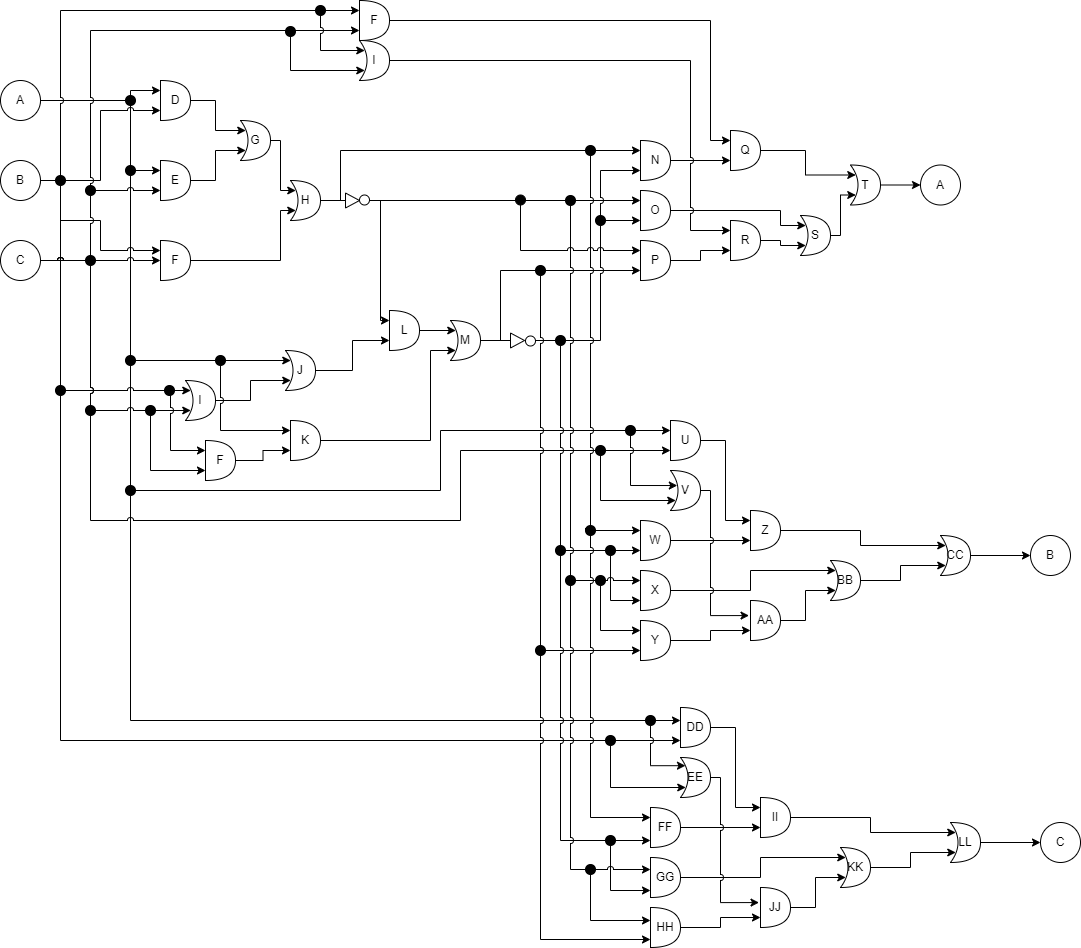
\includegraphics[width = 1\textwidth]{gates.png}
\end{center}

\section{Table}

\begin{center}
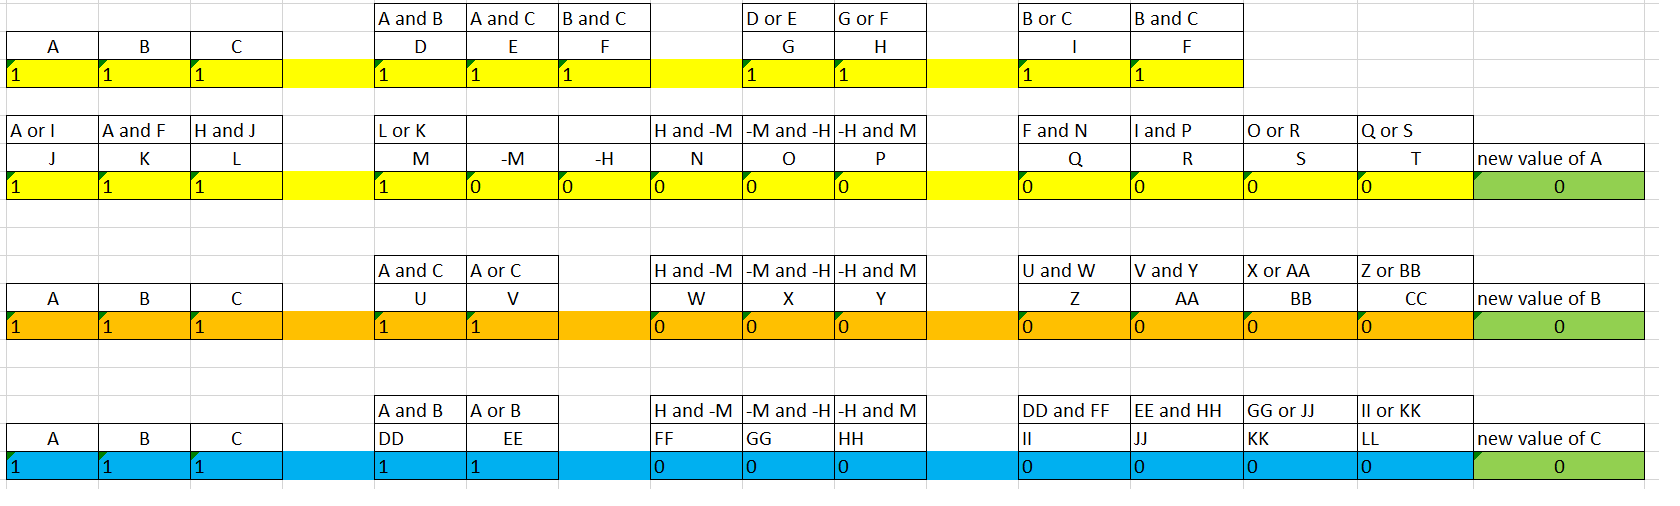
\includegraphics[width = 1\textwidth]{table.png}
\end{center}


\end{document}